\documentclass{article}
\usepackage{amsmath}
\usepackage{graphicx}
\bibliographystyle{IEEEtran}
\usepackage{caption}
\usepackage{subcaption}
\usepackage[colorlinks=true]{hyperref}
\title{Supplemental material for `Eliminating prior-bias from sparse-projection
tomographic reconstructions'}
\begin{document}
\maketitle
This supplementary material consists of details of the optimization routine used in our method, links to view our 3D reconstructions and results of 2D reconstructions for different projection views.

\tableofcontents
\newpage
\section{\textbf{Patch-based techniques}}
\label{sec:patch_based}
Here we present a comparison~\cite{my_dicta_paper} of the performance of the aforementioned PCA-based global prior with a prior that is based on construction of patch-wise dictionaries. In both cases, the reconstruction routine is based on typical CS techniques. The well-known K-SVD algorithm \cite{Aharon2006} was chosen for construction of patch-based dictionaries. For this, patches were extracted from each of the template volumes, from which an overcomplete dictionary was obtained. The basic aim of the K-SVD algorithm (or any overcomplete dictionary learning technique) is the compact linear representation of all these patches using the dictionary columns. Let $\boldsymbol{D}$ denote the dictionary learned, $N_p$ the total number of patches, and $\boldsymbol{H_i}$ the operator to extract the $i^{\textrm{th}}$ patch from the intermediate reconstructed slice/volume. Then, once $\boldsymbol{D}$ is computed in an earlier `training phase', each new test slice (or test volume) can be reconstructed by optimizing a cost function such as the one below:
\begin{multline}
J_2(\boldsymbol{\theta},\{\boldsymbol{\alpha_i}\}_{i=1}^{N_p}) = \lVert\boldsymbol{\mathcal{R}\Upsilon\theta}- \boldsymbol{y}\rVert_2^2  + \lambda_1\lVert\boldsymbol{\theta}\rVert_1 + \\ \frac{\lambda_2}{N_p}\sum_{i=1}^{N_p}\lVert \boldsymbol{H_i\Upsilon \theta}-\boldsymbol{D \alpha_i}\rVert_2^2 +\frac{\lambda_3}{ N_p}\sum_{i=1}^{N_p}\lVert\boldsymbol{\alpha_i}\rVert_1.
\label{Eq:main_patchBased}
\end{multline}
The reconstruction proceeds in an alternating manner, first by minimization of Eq.~\ref{Eq:primaryObj_patchBased} and then by minimization of Eq.~\ref{Eq:alpha_patchBased}. For both these, the solver in~\cite{l1ls} is used. For the former case, the cost function reduces to:
\begin{equation}
J_{\boldsymbol{\alpha}}(\boldsymbol{\theta}) = \lVert \boldsymbol{\mathcal{R} \Upsilon \theta}- \boldsymbol{y}\rVert_2^2  + \lambda_1\lVert\boldsymbol{\theta}\rVert_1 + \frac{\lambda_2}{N_p}\sum_{i=1}^{N_p}\rVert \boldsymbol{H_i \Upsilon \theta}-\boldsymbol{D \alpha_i}\rVert_2^2.
\label{Eq:primaryObj_patchBased}
\end{equation}
For each $i \in \{1,...,N_p\}$, the cost function reduces to:
\begin{equation}
J_{\boldsymbol{\theta}}(\boldsymbol{\alpha}_i) =  \lVert \boldsymbol{H_i \Upsilon \theta}-\boldsymbol{D\alpha_i}\rVert_2^2  + \frac{\lambda_3}{\lambda_2}\lVert\boldsymbol{\alpha_i}\rVert_1.
\label{Eq:alpha_patchBased}
\end{equation}
This summarizes the comparison with patch-based methods.
%--------------------------------------------------------------------------
\section{An alternate method to compute weights-map}
The problem of recovering the unknown data $\boldsymbol{x}$ from its measurements falls under the broad category of inverse problems. In almost all such cases, the measurement model is known. However, a direct analytical inverse solution does not exist in most cases because of the enormous size of the matrix modelling the measurement process. The complexity is further increased when insufficient number of measurements are taken leading to an ill-posed problem. In such circumstances, iterative schemes are used to solve for $\boldsymbol{x}$ by minimizing a cost function. 

A simple cost function $E_\text{model}$ would minimise any difference between the measurements of the data and the imaging model:

\begin{equation}
E_\text{model} = \lVert\boldsymbol{\Phi x- y}\rVert_2^2.
\end{equation}
where $\boldsymbol{y}$ denotes the acquired measurements of $\boldsymbol{x}$ under an imaging model $\boldsymbol{\Phi}$. In our 3D reconstructions, $\boldsymbol{\Phi}$ denotes cone-beam projection model. In the case of sparse measurements (measurements from significantly few projection views), some known information of the underlying unknown data is imposed in order to get its better estimate. The Compressive Sensing is one such method that exploits the fact that most naturally occurring data are sparse under some mathematical transform. The cost function is now given by

\begin{equation}
E_\text{CS} = \lVert\boldsymbol{\Phi x- y}\rVert_2^2  + \lambda_1\lVert\boldsymbol{\theta}\rVert_1
\end{equation}
Here $\boldsymbol{\theta}$ are the unknown sparse coefficients of $\boldsymbol{x}$. In order to further improve the reconstruction, we can use information available from the scans of similar volumes in the past. Such methods are known as `\emph{prior}-based methods'. 

For our reconstruction, the cost function $E$ includes a third term enforcing weighted similarity between the reconstructed volume and pre-computed prior.

\begin{equation}
  E(\boldsymbol{\theta},\boldsymbol{\alpha}) = \lVert\boldsymbol{\Phi x- y}\rVert_2^2  + \lambda_1\lVert\boldsymbol{\theta}\rVert_1 +\lambda_2\lVert\boldsymbol{W}(\boldsymbol{x} - (\boldsymbol{\mu} + \sum_{i}\boldsymbol{V_i}\alpha_i))\rVert_2^2
\label{eq:weighted_prior}
\end{equation}
\newpage



\textbf{Building the prior:}\\

We now describe the method used to build the prior. We begin with, it is assumed that the test volume can be expressed as a compact linear combination of the principal components extracted from a set of similar volumes (called here as `object-prior'). Hence, the prior is built using Principal Component Analysis (PCA), which has been a widely used technique to represent data in terms of its significant modes or directions of variation. \\

First, a set of representative 3D volumes is chosen as object-prior. These volumes must represent a wide range in anatomy, in order to contribute to an eigenspace that can encompass a range of possible test slice anatomy. If these volumes are not aligned, then they must be first registered before computing the prior. The prior is built by computing the covariance matrix $C$ from the template set $\{Q_i\}$, as shown in Eq.~\ref{eq:PCA}, The space spanned by the eigenvectors $\boldsymbol{\{V_i\}}$ (eigenspace) of the covariance matrix is the global prior and is assumed to contain any test slice that is similar, but not necessarily identical to the object-prior. The covariance matrix is given by:
 \begin{equation}
\begin{split}
  C  & = \frac{1}{N-1}\sum_{i=1}^N(Q_i - \mu)(Q_i - \mu)^{T}\\
\end{split}
\label{eq:PCA}
\end{equation}
where $\mu$ denotes the mean of all previously scanned volumes $\{Q_i\}$ and $L$ denotes the number of previously scanned volumes chosen. The eigenvalue decomposition of $C$ will give $L$ orthogonal eigen vectors. We use all of the $L$ eigenvectors as a basis to represent the unknown test volume.  \\

\textbf{Minimizing the Cost function}\\

We minimize the cost specified in Eqn.~\ref{eq:weighted_prior} by alternately solving for $\boldsymbol{\alpha}$ and $\boldsymbol{\theta}$

\begin{equation}
E_{\boldsymbol{\alpha}}(\boldsymbol{\theta}) = ||\Phi\Psi\boldsymbol{\theta}- y||_2^2  + \lambda_1||\boldsymbol{\theta}||_1+\lambda_2||\Psi\boldsymbol{\theta} - (\mu + \sum_{i}V_i\alpha_i)||_2^2
\label{Eq:primaryObj}
\end{equation}
\begin{equation}
E_{\boldsymbol\theta}(\boldsymbol{\alpha}) = ||\Psi\boldsymbol{\theta} - (\mu + \sum_{i}V_i\alpha_i)||_2^2
\label{Eq:alpha1}
\end{equation}
Eq.~\ref{Eq:alpha1} leads to the following closed form update for $\alpha$:
\begin{equation}
\boldsymbol{\alpha} = \boldsymbol{V}^T(\Psi\boldsymbol{\theta} - \mu)
\label{Eq:alpha}
\end{equation}
An optimal value of $\lambda_2$ is empirically chosen \textit{a priori}, based on the reconstructions of one of the template slices.


%--------------------------------Links to videos-------------------------------------------------
\newpage
\section{Links to view our 3D reconstructions}

Please refer to the following videos to view the 3D datasets and reconstruction results referred in our paper:

\begin{itemize}
\item \textbf{Okra groundtruth:} \\ \url{https://www.dropbox.com/s/gn3fk3ev7s7tup0/GroundTruth.mp4?dl=0}\\
	The first four images correspond to the four template volumes and the last (right-most) image corresponds to the test volume.
\item \textbf{Okra 3D reconstruction results:} \\ \url{https://www.dropbox.com/s/o7vga1kjzcayjmt/Reconstruction.mp4?dl=0}\\
       The order of images from left to right correspond to the test volume, FDK reconstruction, CS reconstruction, unselective prior + CS reconstruction, and our reconstruction. 
\item \textbf{Potato groundtruth:} \\ \url{https://www.dropbox.com/s/whwu3th4ozr96k1/GroundTruth.mp4?dl=0}\\
	The first three images correspond to the three template volumes and the last (right-most) image corresponds to the test volume.
\item \textbf{Potato 3D reconstruction results:}\\  \url{https://www.dropbox.com/s/k41qg1kwrry9rwp/Reconstruction.mp4?dl=0}\\
       The order of images from left to right correspond to the test volume, FDK reconstruction, CS reconstruction, unselective prior + CS reconstruction, and our reconstruction.
\item \textbf{Sprouts groundtruth:} \\ \url{https://www.dropbox.com/s/0d7jbojscbx4ciz/GroundTruth.mp4?dl=0}\\
	The first five images correspond to the five template volumes and the last (right-most) image corresponds to the test volume.
\item \textbf{Sprouts 3D reconstruction results:}\\  \url{https://www.dropbox.com/s/o3jmsa4dwtd8a6l/Reconstruction.mp4?dl=0}\\
       The order of images from left to right correspond to the test volume, FDK reconstruction, CS reconstruction, unselective prior + CS reconstruction, and our reconstruction.

\end{itemize}

\newpage
\section{2D reconstruction results on colon CT dataset}

\begin{figure}[h]
    \begin{subfigure}[b]{0.3\linewidth}
        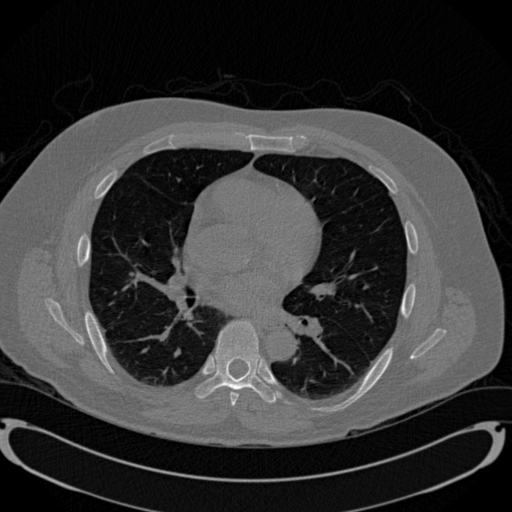
\includegraphics[width=\textwidth]{../images/supplementary/colon/template1.png}
        \caption{template 1}
    \end{subfigure}
    \begin{subfigure}[b]{0.3\linewidth}
        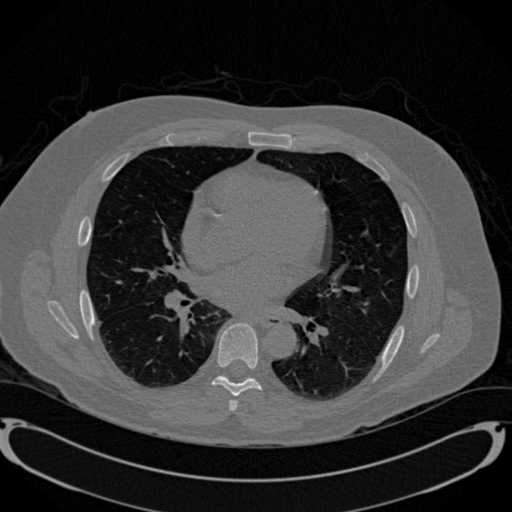
\includegraphics[width=\textwidth]{../images/supplementary/colon/template2.png}
        \caption{template 2}
     \end{subfigure}
    \begin{subfigure}[b]{0.3\linewidth}
        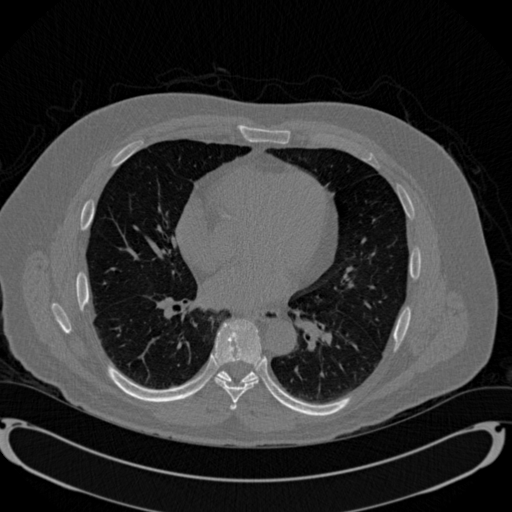
\includegraphics[width=\textwidth]{../images/supplementary/colon/template3.png}
        \caption{template 3}
     \end{subfigure}
    \begin{subfigure}[b]{0.3\linewidth}
        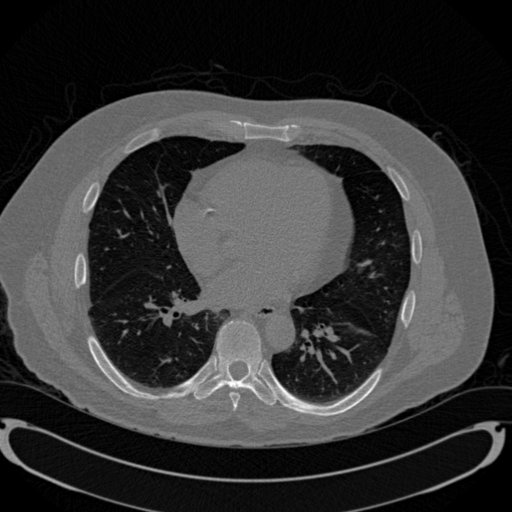
\includegraphics[width=\textwidth]{../images/supplementary/colon/template4.png}
        \caption{template 4}
     \end{subfigure}
\quad
    \begin{subfigure}[b]{0.3\linewidth}
        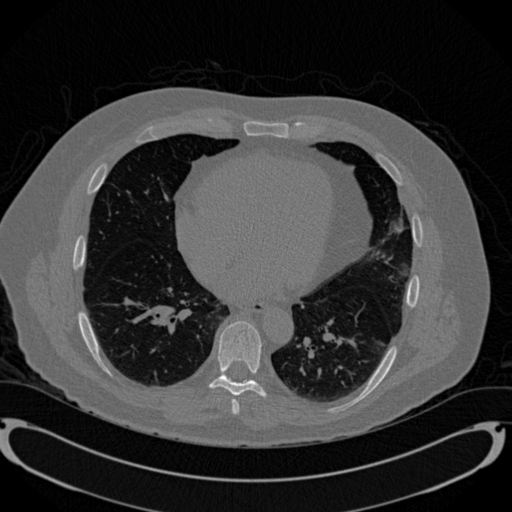
\includegraphics[width=\textwidth]{../images/supplementary/colon/template5.png}
        \caption{template 5}
     \end{subfigure}
\quad
    \begin{subfigure}[b]{0.3\linewidth}
        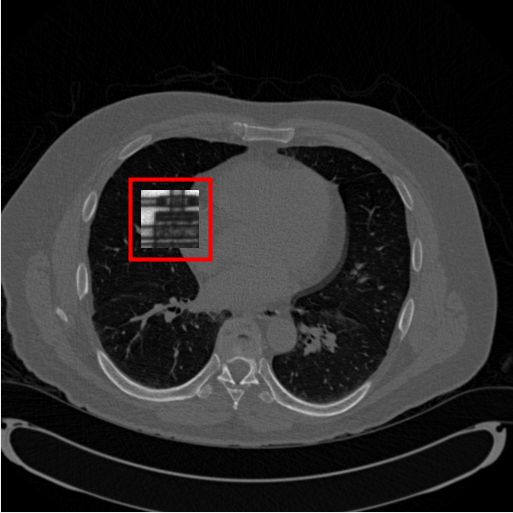
\includegraphics[width=\textwidth]{../images/supplementary/colon/testIm.png}
        \caption{test image}
     \end{subfigure}
      \caption{2D object-prior (referred to as `templates' here)  and test slice of colon CT dataset. The region in red shows the synthetic new region added to the test slice.}
\label{fig:joint}
\end{figure}

%--------------------------------2D Colon results----------------------------

\newpage
\begin{figure}[h]
    \begin{subfigure}[b]{0.3\linewidth}
        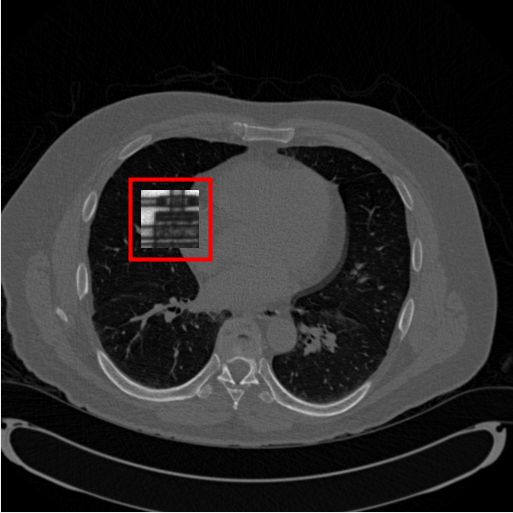
\includegraphics[width=\textwidth]{../images/supplementary/colon/testIm.png}
        \caption{Test image}
     \end{subfigure}
    \begin{subfigure}[b]{0.3\linewidth}
        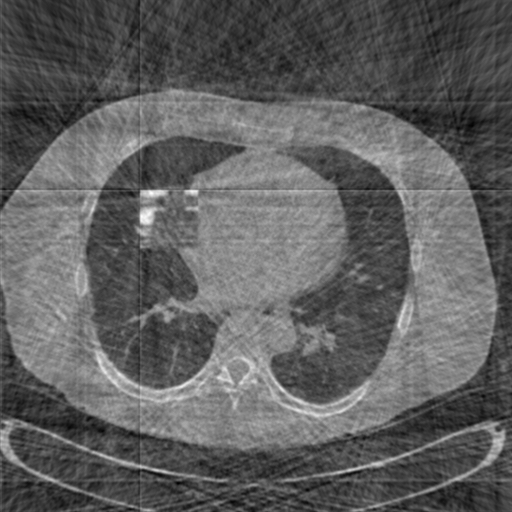
\includegraphics[width=\textwidth]{../images/supplementary/colon/60_angles/fbp.png}
        \caption{FBP}
    \end{subfigure}
    \begin{subfigure}[b]{0.3\linewidth}
        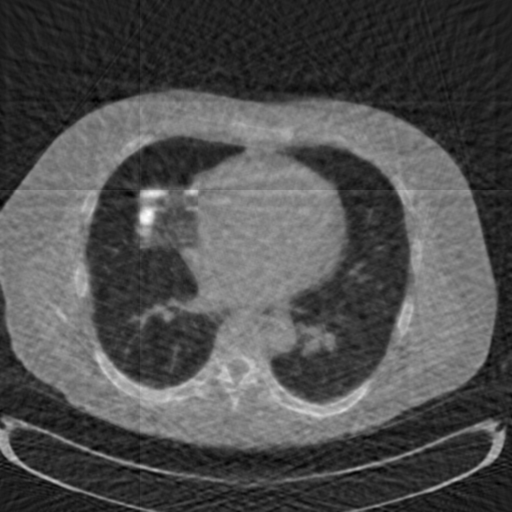
\includegraphics[width=\textwidth]{../images/supplementary/colon/60_angles/cs_dct.png}
        \caption{CS-DCT}
     \end{subfigure}
    \begin{subfigure}[b]{0.3\linewidth}
        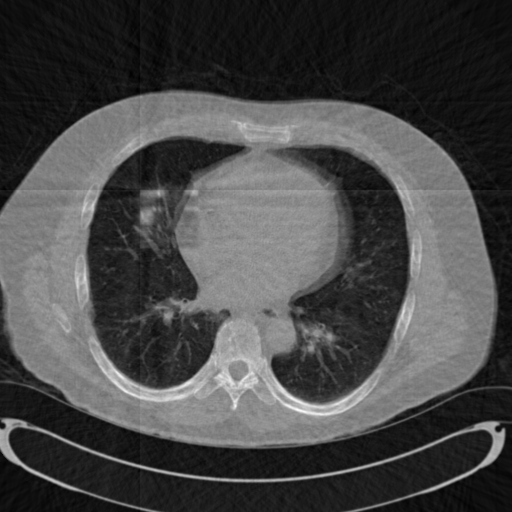
\includegraphics[width=\textwidth]{../images/supplementary/colon/60_angles/plain_pca.png}
        \caption{unselective prior+cs}
     \end{subfigure}
\quad
    \begin{subfigure}[b]{0.3\linewidth}
        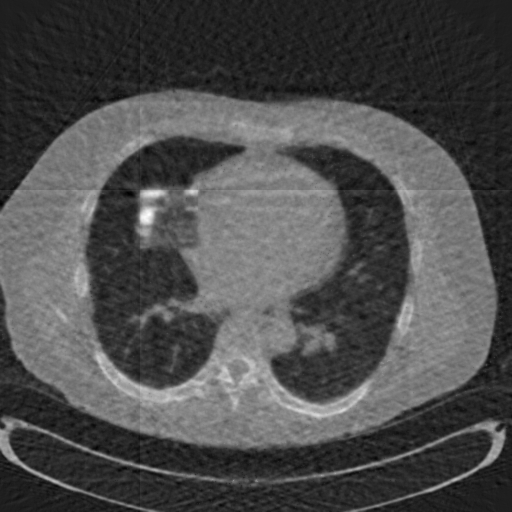
\includegraphics[width=\textwidth]{../images/supplementary/colon/60_angles/weighted_pca5.png}
       \caption{our method}
     \end{subfigure}
      \caption{Reconstruction of colon CT: (b) has many streak artefacts (c) slightly blurred (d) Inaccurate reconstruction of new region (corresponding to the red RoI) (d) new region accurately detected while simultaneously removing streak artefacts.}
\label{fig:joint}
\end{figure}


%-----------------------------Sprouts : data--------------------------
\newpage
\section{2D reconstruction for different projection views}

\textbf{2D Sprouts dataset}

\begin{figure}[h]
    \begin{subfigure}[b]{0.3\linewidth}
        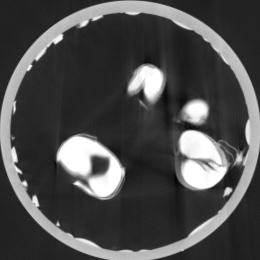
\includegraphics[width=\textwidth]{../images/supplementary/2D_sprouts/template1.png}
        \caption{template 1}
    \end{subfigure}
    \begin{subfigure}[b]{0.3\linewidth}
        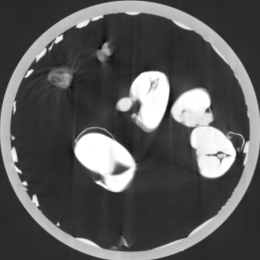
\includegraphics[width=\textwidth]{../images/supplementary/2D_sprouts/template2.png}
        \caption{template 2}
     \end{subfigure}
    \begin{subfigure}[b]{0.3\linewidth}
        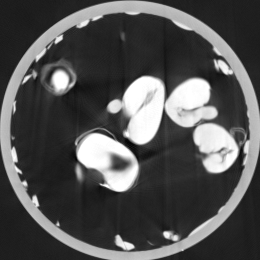
\includegraphics[width=\textwidth]{../images/supplementary/2D_sprouts/template3.png}
        \caption{template 3}
     \end{subfigure}
    \begin{subfigure}[b]{0.3\linewidth}
        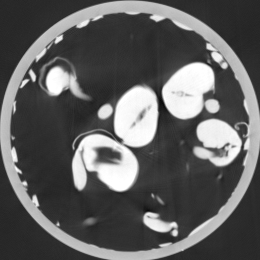
\includegraphics[width=\textwidth]{../images/supplementary/2D_sprouts/template4.png}
        \caption{template 4}
     \end{subfigure}
\quad
    \begin{subfigure}[b]{0.3\linewidth}
        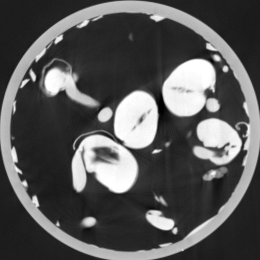
\includegraphics[width=\textwidth]{../images/supplementary/2D_sprouts/template5.png}
        \caption{template 5}
     \end{subfigure}
\quad
    \begin{subfigure}[b]{0.3\linewidth}
        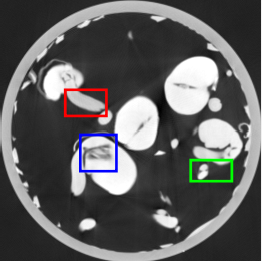
\includegraphics[width=\textwidth]{../images/supplementary/2D_sprouts/colorTestIm.png}
        \caption{test image}
     \end{subfigure}
      \caption{Sprouts data: CT of different stages of sprouts growing in a jar. The templates refer to previously scanned volumes that form the `object-prior'.}
\label{fig:joint}
\end{figure}

%-----------------------------Sprouts (19 angles)--------------------------
\newpage
\subsection{Reconstruction from 19 projection views}
\begin{figure}[h]
    \begin{subfigure}[b]{0.3\linewidth}
        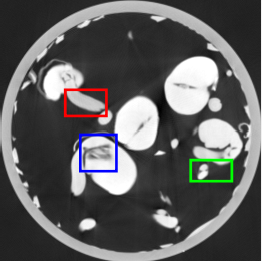
\includegraphics[width=\textwidth]{../images/supplementary/2D_sprouts/colorTestIm.png}
        \caption{Test image}
     \end{subfigure}
    \begin{subfigure}[b]{0.3\linewidth}
        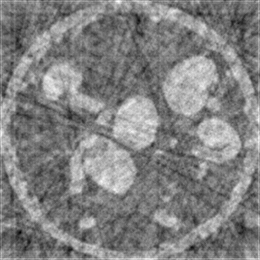
\includegraphics[width=\textwidth]{../images/supplementary/2D_sprouts/19_angles/1/fbp.png}
        \caption{FBP}
    \end{subfigure}
    \begin{subfigure}[b]{0.3\linewidth}
        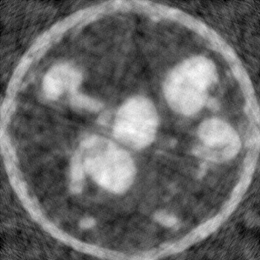
\includegraphics[width=\textwidth]{../images/supplementary/2D_sprouts/19_angles/1/cs_dct.png}
        \caption{CS-DCT}
     \end{subfigure}
    \begin{subfigure}[b]{0.3\linewidth}
        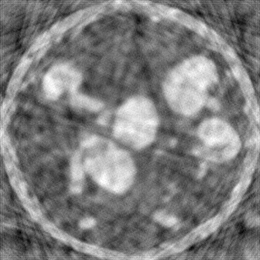
\includegraphics[width=\textwidth]{../images/supplementary/2D_sprouts/19_angles/1/cs_wavelet.png}
        \caption{CS-wavelet}
     \end{subfigure}
\quad
    \begin{subfigure}[b]{0.3\linewidth}
        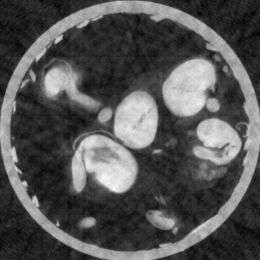
\includegraphics[width=\textwidth]{../images/supplementary/2D_sprouts/19_angles/1/plain_pca.png}
        \caption{unselective prior+cs}
     \end{subfigure}
\quad
    \begin{subfigure}[b]{0.3\linewidth}
        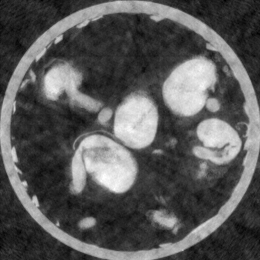
\includegraphics[width=\textwidth]{../images/supplementary/2D_sprouts/19_angles/1/weighted_pca5.png}
       \caption{our method}
     \end{subfigure}
      \caption{Reconstruction of sprouts [260 x 260] image from measurements obtained by $10\%$ sampling (19 projection views).}
\label{fig:joint}
\end{figure}

%-----------------------------Sprouts (66 angles)--------------------------
\newpage
\subsection{Reconstruction from 66 projection views}
\begin{figure}[h]
    \begin{subfigure}[b]{0.3\linewidth}
        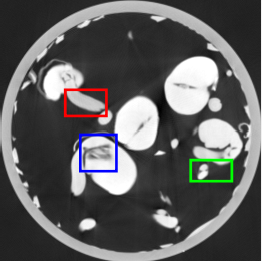
\includegraphics[width=\textwidth]{../images/supplementary/2D_sprouts/colorTestIm.png}
        \caption{Test image}
     \end{subfigure}
    \begin{subfigure}[b]{0.3\linewidth}
        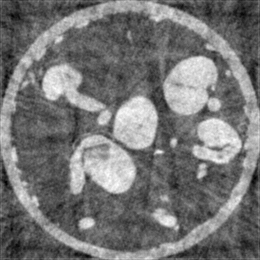
\includegraphics[width=\textwidth]{../images/supplementary/2D_sprouts/55_angles/1/fbp.png}
        \caption{FBP}
    \end{subfigure}
    \begin{subfigure}[b]{0.3\linewidth}
        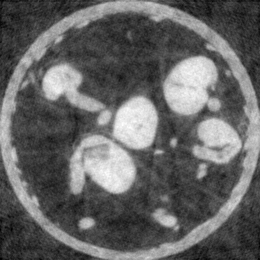
\includegraphics[width=\textwidth]{../images/supplementary/2D_sprouts/55_angles/1/cs_dct.png}
        \caption{CS-DCT}
     \end{subfigure}
    \begin{subfigure}[b]{0.3\linewidth}
        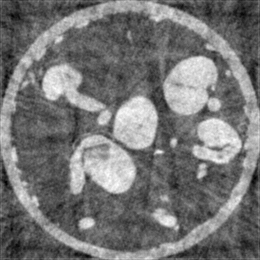
\includegraphics[width=\textwidth]{../images/supplementary/2D_sprouts/55_angles/1/cs_wavelet.png}
        \caption{CS-wavelet}
     \end{subfigure}
\quad
    \begin{subfigure}[b]{0.3\linewidth}
        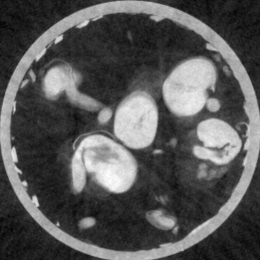
\includegraphics[width=\textwidth]{../images/supplementary/2D_sprouts/55_angles/1/plain_pca.png}
        \caption{unselective prior+cs}
     \end{subfigure}
\quad
    \begin{subfigure}[b]{0.3\linewidth}
        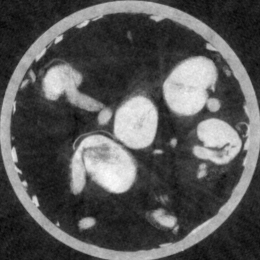
\includegraphics[width=\textwidth]{../images/supplementary/2D_sprouts/55_angles/1/weighted_pca5.png}
        \caption{our method}
     \end{subfigure}
     \caption{Reconstruction of sprouts [260 x 260] image from measurements obtained by $30\%$ sampling (55 projection views).} 
\label{fig:joint}
\end{figure}

%-----------------------------Sprouts (110 angles)--------------------------
\newpage
\subsection{Reconstruction from 110 projection views}
\begin{figure}[h]
    \begin{subfigure}[b]{0.3\linewidth}
        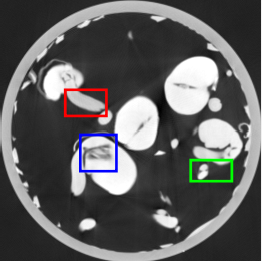
\includegraphics[width=\textwidth]{../images/supplementary/2D_sprouts/colorTestIm.png}
        \caption{Test image}
     \end{subfigure}
    \begin{subfigure}[b]{0.3\linewidth}
        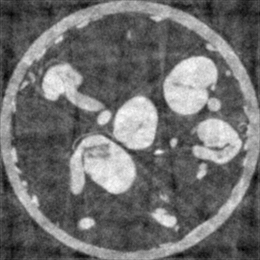
\includegraphics[width=\textwidth]{../images/supplementary/2D_sprouts/92_angles/1/fbp.png}
        \caption{FBP}
    \end{subfigure}
    \begin{subfigure}[b]{0.3\linewidth}
        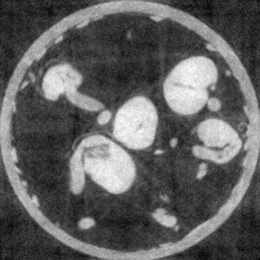
\includegraphics[width=\textwidth]{../images/supplementary/2D_sprouts/92_angles/1/cs_dct.png}
        \caption{CS-DCT}
     \end{subfigure}
    \begin{subfigure}[b]{0.3\linewidth}
        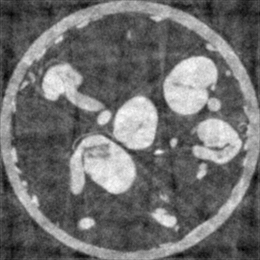
\includegraphics[width=\textwidth]{../images/supplementary/2D_sprouts/92_angles/1/cs_wavelet.png}
        \caption{CS-wavelet}
     \end{subfigure}
\quad
    \begin{subfigure}[b]{0.3\linewidth}
        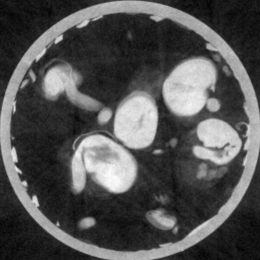
\includegraphics[width=\textwidth]{../images/supplementary/2D_sprouts/92_angles/1/plain_pca.png}
        \caption{unselective prior}
     \end{subfigure}
\quad
    \begin{subfigure}[b]{0.3\linewidth}
        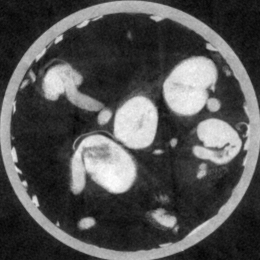
\includegraphics[width=\textwidth]{../images/supplementary/2D_sprouts/92_angles/1/weighted_pca5.png}
        \caption{our method}
     \end{subfigure}
     \caption{Reconstruction of sprouts [260 x 260] image from measurements obtained by $50\%$ sampling (92 projection views).} 
\label{fig:joint}
\end{figure}

%-----------------------------Sprouts (154 angles)--------------------------
\newpage
\subsection{Reconstruction from 154 projection views}
\begin{figure}[h]
    \begin{subfigure}[b]{0.3\linewidth}
        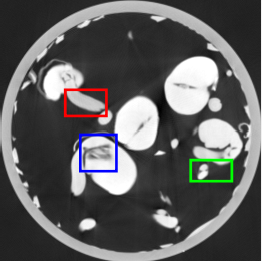
\includegraphics[width=\textwidth]{../images/supplementary/2D_sprouts/colorTestIm.png}
        \caption{Test image}
     \end{subfigure}
    \begin{subfigure}[b]{0.3\linewidth}
        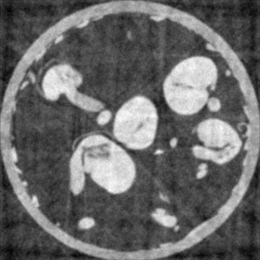
\includegraphics[width=\textwidth]{../images/supplementary/2D_sprouts/154_angles/1/fbp.png}
        \caption{FBP}
    \end{subfigure}
    \begin{subfigure}[b]{0.3\linewidth}
        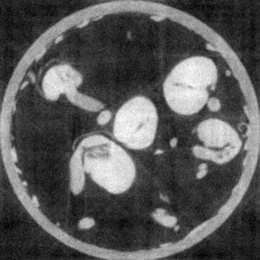
\includegraphics[width=\textwidth]{../images/supplementary/2D_sprouts/154_angles/1/cs_dct.png}
        \caption{CS-DCT}
     \end{subfigure}
    \begin{subfigure}[b]{0.3\linewidth}
        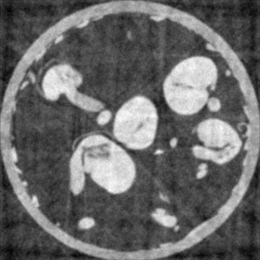
\includegraphics[width=\textwidth]{../images/supplementary/2D_sprouts/154_angles/1/cs_wavelet.png}
        \caption{CS-wavelet}
     \end{subfigure}
\quad
    \begin{subfigure}[b]{0.3\linewidth}
        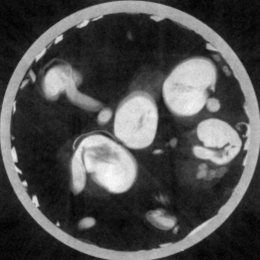
\includegraphics[width=\textwidth]{../images/supplementary/2D_sprouts/154_angles/1/plain_pca.png}
        \caption{prior unselective+cs}
     \end{subfigure}
\quad
    \begin{subfigure}[b]{0.3\linewidth}
        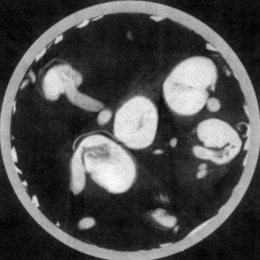
\includegraphics[width=\textwidth]{../images/supplementary/2D_sprouts/154_angles/1/weighted_pca5.png}
        \caption{our method}
     \end{subfigure}
     \caption{Reconstruction of sprouts [260 x 260] image from measurements obtained by $83\%$ sampling (154 projection views).} 
\label{fig:joint}
\end{figure}
\newpage
%--------------------------BIG images: TMH results
\section{Bigger images for reconstruction results shown in main paper}
\subsection{Liver}
%-------RFA2 moderate views
\textbf{Goal: Observe details of new changes}
\begin{figure}[!h]
\centering
\subcaptionbox{Test}{\fcolorbox{white}{blue}{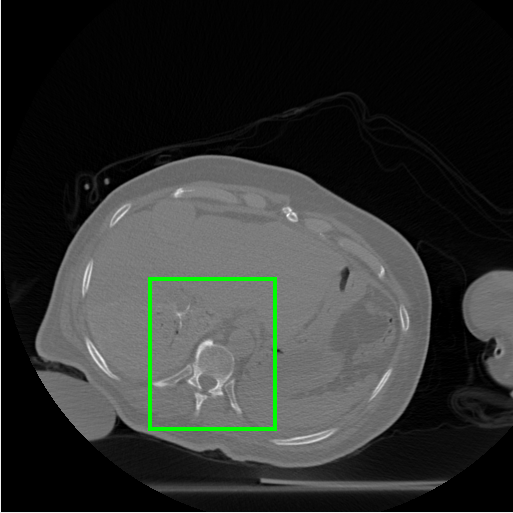
\includegraphics[width=0.49\columnwidth]{../images/tmh/RFA2/few_views/colorTestIm.png}}}\hfill
\subcaptionbox{FBP}{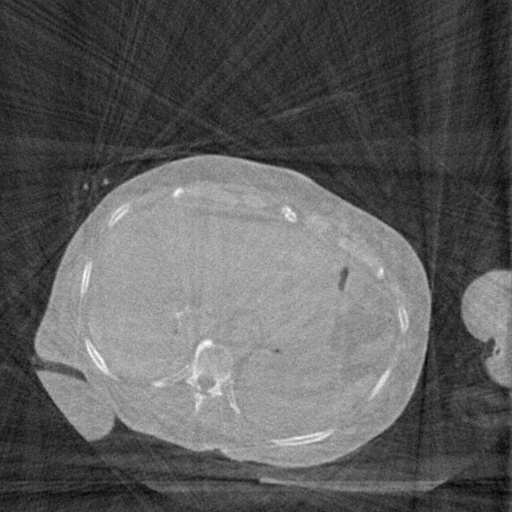
\includegraphics[width=0.49\columnwidth]{../images/tmh/RFA2/few_views/fbp.png}}\hfill
\subcaptionbox{l1-ls}{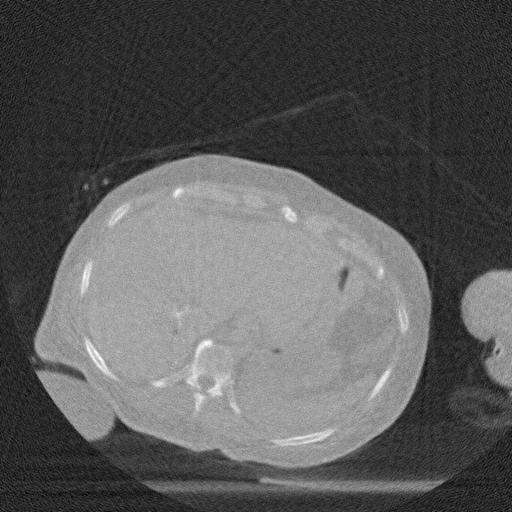
\includegraphics[width=0.49\columnwidth]{../images/tmh/RFA2/few_views/cs_dct.png}}\hfill
\subcaptionbox{Spatially-varying prior}{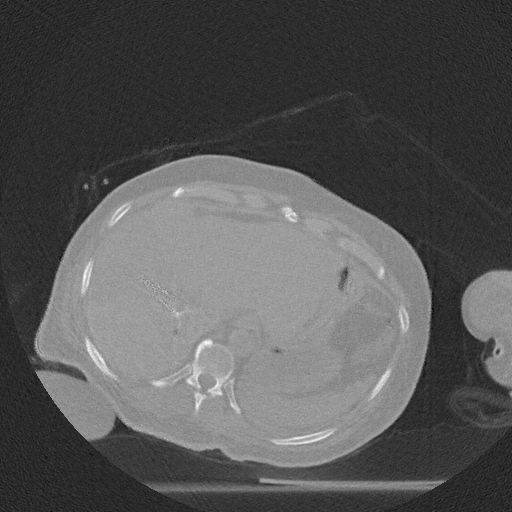
\includegraphics[width=0.49\columnwidth]{../images/tmh/RFA2/few_views/weighted_pca_all_methods_kk_0_01.png}}
\caption[Representative results-2]{Reconstruction of Liver corresponding to Figure 8 of the main paper.}
\label{fig:RFA2_few_views_biggerIm}
\end{figure}
\newpage

\textbf{Test image Figure~\ref{fig:RFA2_few_views_biggerIm}  is shown in larger display here  again for better clarity.}\\
\begin{figure}[!h]
\centering
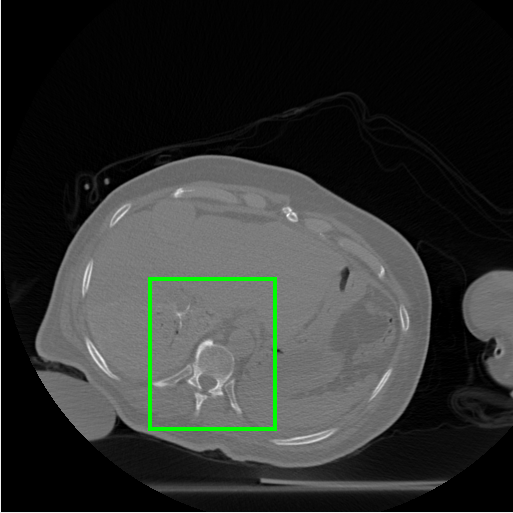
\includegraphics[width=1.2\columnwidth]{../images/tmh/RFA2/few_views/colorTestIm.png}
\captionsetup{labelformat=empty}
\caption[Representative results-2]{\large{Test slice}}
\label{fig:RFA2_few_views_bigger}
\end{figure}
\newpage
\textbf{Reconstruction result of Figure~\ref{fig:RFA2_few_views_biggerIm}  is shown in larger display here  again for better clarity.}\\
\begin{figure}[!h]
\centering
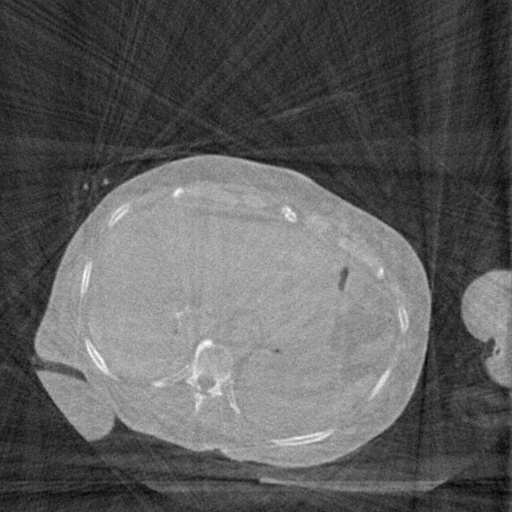
\includegraphics[width=1.2\columnwidth]{../images/tmh/RFA2/few_views/fbp.png}
\captionsetup{labelformat=empty}
\caption[Representative results-2]{\large{FBP}}
\label{fig:RFA2_few_views_bigger}
\end{figure}
\newpage
\textbf{Reconstruction result of Figure~\ref{fig:RFA2_few_views_biggerIm}  is shown in larger display here  again for better clarity.}\\
\begin{figure}[!h]
\centering
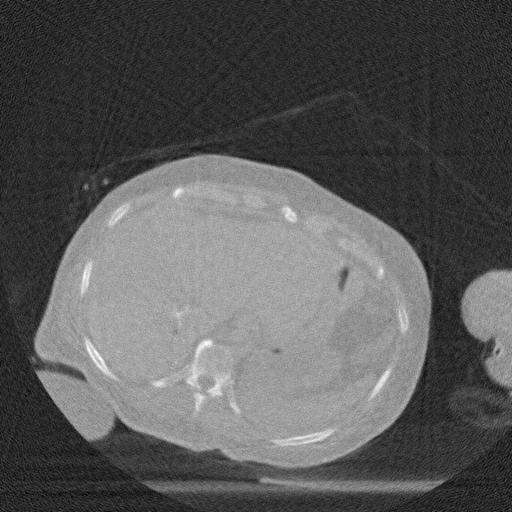
\includegraphics[width=1.2\columnwidth]{../images/tmh/RFA2/few_views/cs_dct.png}
\captionsetup{labelformat=empty}
\caption[Representative results-2]{\large{l1-ls}}
\label{fig:RFA2_few_views_bigger}
\end{figure}
\newpage
\textbf{Reconstruction result of Figure~\ref{fig:RFA2_few_views_biggerIm} is shown in larger display here  again for better clarity.}\\
\begin{figure}[!h]
\centering
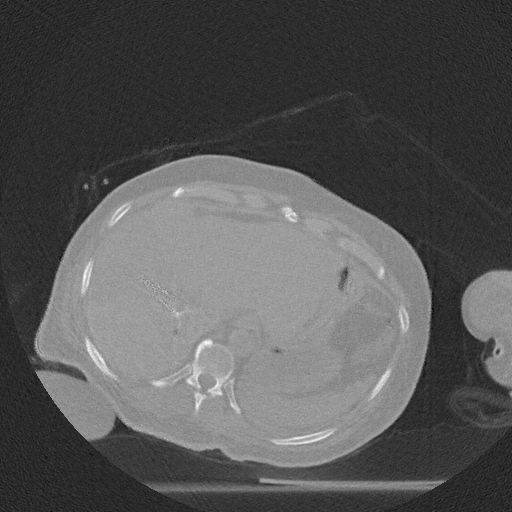
\includegraphics[width=1.2\columnwidth]{../images/tmh/RFA2/few_views/weighted_pca_all_methods_kk_0_01.png}
\captionsetup{labelformat=empty}
\caption[Representative results-2]{\large{Spatially-varying prior method}}
\label{fig:RFA2_few_views_bigger}
\end{figure}
\newpage

%------------------------------------Bigger images for Sprouts------------------
\textbf{Sprouts:}

\begin{figure}[!h]
    \begin{subfigure}[b]{0.4\linewidth}
        \fcolorbox{green}{green}{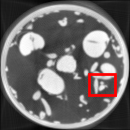
\includegraphics[width=\textwidth]{../images/sprouts/testIm_red.png}}
%\captionsetup{labelformat=empty}
        \caption{Test}
     \end{subfigure}
\quad
    \begin{subfigure}[b]{0.4\linewidth}
        \includegraphics[width=\textwidth]{../images/sprouts/fdkIm.png}
%\captionsetup{labelformat=empty}
        \caption{FDK}
    \end{subfigure}
\quad
    \begin{subfigure}[b]{0.4\linewidth}
        \includegraphics[width=\textwidth]{../images/sprouts/csIm.png}
%\captionsetup{labelformat=empty}
        \caption{l1-ls}
     \end{subfigure}\\
\quad
    \begin{subfigure}[b]{0.4\linewidth}
        \includegraphics[width=\textwidth]{../images/sprouts/plainPriorIm.png}
%\captionsetup{labelformat=empty}
        \caption{Uniform\\ Prior}
     \end{subfigure}
\quad
    \begin{subfigure}[b]{0.4\linewidth}
        \includegraphics[width=\textwidth]{../images/sprouts/weightedPriorIm.png}
%\captionsetup{labelformat=empty}
        \caption{Spatially-Varying\\ prior}
    \end{subfigure}
    %\quad
    %\captionsetup{labelformat=empty}
     \caption{Reconstruction of sprouts corresponding to Figure 16 of the main paper.} 
\label{fig:sprouts_3D_results_biggerIm}
%\addtolength{\textfloatsep}{-0.8cm}
\end{figure}

\newpage
\textbf{Test image of Figure~\ref{fig:sprouts_3D_results_biggerIm}  is shown in larger display here  again for better clarity.}\\
\begin{figure}[!h]
    \begin{subfigure}[b]{\linewidth}
        \fcolorbox{green}{green}{\includegraphics[width=\textwidth]{../images/sprouts/testIm_red.png}}
\captionsetup{labelformat=empty}
        \caption{\large{Test}}
     \end{subfigure}
\end{figure}
\newpage
\textbf{Reconstruction result of Figure~\ref{fig:sprouts_3D_results_biggerIm}  is shown in larger display here  again for better clarity.}\\
\begin{figure}[!h]
    \begin{subfigure}[b]{\linewidth}
        \fcolorbox{green}{green}{\includegraphics[width=\textwidth]{../images/sprouts/fdkIm.png}}
\captionsetup{labelformat=empty}
        \caption{\large{FDK}}
     \end{subfigure}
\end{figure}
\newpage
\textbf{Reconstruction result of Figure~\ref{fig:sprouts_3D_results_biggerIm}  is shown in larger display here  again for better clarity.}\\
\begin{figure}[!h]
    \begin{subfigure}[b]{\linewidth}
        \fcolorbox{green}{green}{\includegraphics[width=\textwidth]{../images/sprouts/csIm.png}}
\captionsetup{labelformat=empty}
        \caption{\large{l1-ls}}
     \end{subfigure}
\end{figure}
\newpage
\textbf{Reconstruction result of Figure~\ref{fig:sprouts_3D_results_biggerIm}  is shown in larger display here  again for better clarity.}\\
\begin{figure}[!h]
    \begin{subfigure}[b]{\linewidth}
        \fcolorbox{green}{green}{\includegraphics[width=\textwidth]{../images/sprouts/plainPriorIm.png}}
\captionsetup{labelformat=empty}
        \caption{\large{Uniform Prior}}
     \end{subfigure}
\end{figure}
\newpage
\textbf{Reconstruction result of Figure~\ref{fig:sprouts_3D_results_biggerIm}  is shown in larger display here  again for better clarity.}\\
\begin{figure}[!h]
    \begin{subfigure}[b]{\linewidth}
        \fcolorbox{green}{green}{\includegraphics[width=\textwidth]{../images/sprouts/weightedPriorIm.png}}
\captionsetup{labelformat=empty}
        \caption{\large{Spatially-Varying Prior}}
     \end{subfigure}
\end{figure}
\newpage

%--------------------------------Bigger results for Okra------------------------
\textbf{Okra:}

\begin{figure}[!h]
\centering
\subcaptionbox{Test}{\fcolorbox{yellow}{yellow}{\includegraphics[width=0.2\columnwidth]{../images/okra/testCropped.png}}}\hfill
\subcaptionbox{FDK, no prior}{\includegraphics[width=0.2\columnwidth]{../images/okra/fdk_cropped.png}}\hfill
\subcaptionbox{l1-ls}{\includegraphics[width=0.2\columnwidth]{../images/okra/cs_cropped.png}}\hfill
\subcaptionbox{\mbox{Uniform}\\prior}{\includegraphics[width=0.2\columnwidth]{../images/okra/pca_cropped.png}}\hfill
\subcaptionbox{Spatially-Varying\\ prior}{\includegraphics[width=0.2\columnwidth]{../images/okra/prior_weighted_cropped.png}}
\caption{Reconstruction of okra corresponding to Figure 14 of the main paper.}
\label{fig:okra_3D_results_biggerIm}
\end{figure}
\newpage
\textbf{Test image of Figure~\ref{fig:okra_3D_results_biggerIm}  is shown in larger display here  again for better clarity.}
\begin{figure}[!h]
\centering
       \includegraphics[width=0.5\columnwidth]{../images/okra/testCropped.png}
\captionsetup{labelformat=empty}
        \caption{\large{Test}}
\end{figure}
\newpage

\textbf{Reconstruction result of Figure~\ref{fig:okra_3D_results_biggerIm}  is shown in larger display here  again for better clarity.}
\begin{figure}[!h]
\centering
       \includegraphics[width=0.5\columnwidth]{../images/okra/fdk_cropped.png}
\captionsetup{labelformat=empty}
        \caption{\large{FDK}}
\end{figure}
\newpage

\textbf{Reconstruction result of Figure~\ref{fig:okra_3D_results_biggerIm}  is shown in larger display here  again for better clarity.}
\begin{figure}[!h]
\centering
       \includegraphics[width=0.5\columnwidth]{../images/okra/cs_cropped.png}
\captionsetup{labelformat=empty}
        \caption{\large{l1-ls}}
\end{figure}
\newpage


\textbf{Reconstruction result of Figure~\ref{fig:okra_3D_results_biggerIm}  is shown in larger display here  again for better clarity.}
\begin{figure}[!h]
\centering
       \includegraphics[width=0.5\columnwidth]{../images/okra/pca_cropped.png}
\captionsetup{labelformat=empty}
        \caption{\large{Uniform Prior}}
\end{figure}
\newpage

\textbf{Reconstruction result of Figure~\ref{fig:okra_3D_results_biggerIm}  is shown in larger display here  again for better clarity.}
\begin{figure}[!h]
\centering
       \includegraphics[width=0.5\columnwidth]{../images/okra/prior_weighted_cropped.png}
\captionsetup{labelformat=empty}
        \caption{\large{Spatially-Varying prior}}
\end{figure}
\newpage

%----------------------------------Comparison with Literature------------------------
\section{Detecting new changes directly in the measurements}
Sec.2 of the main paper (`Related work') contrasts the spatially-varying technique  with other prior based techniques in literature. Here we present a 2D reconstruction  result (of the test shown in Figure.~\ref{fig:comparisonLit_dataset}) to compare our method with~\cite{Lee2012}, in which the new changes are directly detected in the measurement space by computing the difference between the measurements of the test and the corresponding simulated measurements of the template. This difference-volume is then reconstructed and then fused (added to) with the original high quality template. However, in the above method, the sub-sampling artefacts present in the difference-volume gets carried over to the final reconstructed image. This is shown in Figure~\ref{fig:comparisonLit_results}. A quantitative comparison over the region of interest is shown in Table~\ref{tab:comparisonLit}.
\begin{figure}[!h]
    \begin{subfigure}[b]{0.4\linewidth}
        \includegraphics[width=\textwidth]{../images/potato/template_3.png}
%\captionsetup{labelformat=empty}
        \caption{Template}
     \end{subfigure}
\quad
    \begin{subfigure}[b]{0.4\linewidth}
        \includegraphics[width=\textwidth]{../images/potato/testIm_color.png}
%\captionsetup{labelformat=empty}
        \caption{Test}
    \end{subfigure}
    %\captionsetup{labelformat=empty}
     \caption{Template and test from the Potato dataset for the reconstructions shown in Figure.~\ref{fig:comparisonLit_results}} 
\label{fig:comparisonLit_dataset}
%\addtolength{\textfloatsep}{-0.8cm}
\end{figure}
\newpage

\begin{figure}[!h]
    \begin{subfigure}[b]{0.4\linewidth}
        \includegraphics[width=\textwidth]{../images/comparison_lit/result_new_changes.png}
%\captionsetup{labelformat=empty}
        \caption{~\cite{Lee2012}:new-changes}
     \end{subfigure}
\quad
    \begin{subfigure}[b]{0.4\linewidth}
        \includegraphics[width=\textwidth]{../images/comparison_lit/result_literature_test.png}
%\captionsetup{labelformat=empty}
        \caption{~\cite{Lee2012}:Reconstruction}
    \end{subfigure}

    \begin{subfigure}[b]{0.4\linewidth}
        \includegraphics[width=\textwidth]{../images/comparison_lit/weightsIm_all_methods30.png}
%\captionsetup{labelformat=empty}
        \caption{Our weights-map}
    \end{subfigure}
   \quad
        \begin{subfigure}[b]{0.4\linewidth}
        \includegraphics[width=\textwidth]{../images/comparison_lit/weighted_pca_all_methods30.png}
%\captionsetup{labelformat=empty}
        \caption{Our Reconstruction}
    \end{subfigure}
    %\captionsetup{labelformat=empty}
     \caption{Reconstruction of the test in Figure~\ref{fig:comparisonLit_dataset}.  Reconstructions were performed from 12 views. Gaussian noise of 0 mean and SD = $1\%$ of mean of measurements, was added to the measurements.} 
\label{fig:comparisonLit_results}
%\addtolength{\textfloatsep}{-0.8cm}
\end{figure}

\begin{table}[!h]
  \centering
      \caption{SSIM values (within RoI) of reconstructions shown in Figure~\ref{fig:comparisonLit_results}}
  \begin{tabular}{|l|l|l|}
\hline
 & \textbf{SSIM (whole image)} & \textbf{SSIM (RoI)} \\ \hline
\textbf{Method in~\cite{Lee2012}} & 0.65 & 0.60 \\ \hline
\textbf{\begin{tabular}[c]{@{}l@{}}Spatially-varying \\prior\end{tabular}} & 0.89 & 0.92 \\ \hline
  \end{tabular}
  \label{tab:comparisonLit}
\end{table}

\bibliography{tci_ref}
\end{document}

